\pdfminorversion=6
\documentclass[xcolor=table]{beamer}
%\newcommand{\pagelogo}{ru/logo.png}
%\newcommand{\bannerlogo}{ru/logo.png}

\usepackage{svg}
\usepackage{lmodern,amsmath,amssymb}
\usepackage{adjustbox}
\usepackage{mathtools}
\usepackage{algpseudocode}
\usepackage[customcolors]{hf-tikz}
\usetheme{Warsaw}
\setbeamertemplate{enumerate items}[default]
\setbeamerfont{enumerate item}{series=\bfseries\itshape}
\usecolortheme{beaver}
\usefonttheme[onlymath]{serif}
\usepackage[T1]{fontenc} %  fontenc is used to fix the bug for greek letter \Delta
\usepackage{arydshln}
\usepackage{cancel}
\usepackage{blkarray, bigstrut}
\usepackage{accents}
\usepackage{listings}
\usepackage{multicol}
\usepackage{hyperref}
\usepackage{tikz}
\usepackage{graphicx}
\setlength\columnsep{15pt}
\usepackage{makecell}
\renewcommand{\arraystretch}{1.2}


%% customization of beamer environments
%% copyright notice
\setbeamertemplate{footline}{%
	\leavevmode%
	\hbox{\begin{beamercolorbox}[wd=.5\paperwidth,ht=2.0ex,dp=2.125ex,leftskip=.3cm plus1fill,rightskip=.3cm]{author in head/foot}%
			\usebeamerfont{author in head/foot}\copyright Dov Kruger 2024\vspace{-1ex}
		\end{beamercolorbox}%
		\begin{beamercolorbox}[wd=.5\paperwidth,ht=2.0ex,dp=2.125ex,leftskip=.3cm,rightskip=.3cm plus1fil]{title in head/foot}%
			\usebeamerfont{title in head/foot}{\insertshorttitle}\vspace{-1ex}
	\end{beamercolorbox}}%
	\vskip0pt%
}
%% logo banner
\setbeamertemplate{background canvas}{%
	\raisebox{-\paperheight+10pt}[0pt][0pt]{%
		\makebox[\paperwidth][l]{%
			\hspace{1cm}
\includegraphics[width=1.5cm]{ru/logo.png}%
		}%
	}%
}
%% create an environment called "withoutheadline" to save space on content slides
\makeatletter
\newenvironment{withoutheadline}{
	\setbeamertemplate{headline}[default]
	\def\beamer@entrycode{\vspace*{-\headheight}}
	\setbeamertemplate{background canvas}{%
		\raisebox{-\paperheight+\headheight+10pt}[0pt][0pt]{%
			\makebox[\paperwidth][l]{%
				\hspace{.5cm}
\includegraphics[width=1cm]{ru/logo.png}%
			}%
		}%
	}
}{}
\makeatother
%% create an environment called "withoutheadlinelogoright" in which the logo is located on the right
\makeatletter
\newenvironment{withoutheadlinelogoright}{
	\setbeamertemplate{headline}[default]
	\def\beamer@entrycode{\vspace*{-\headheight}}
	\setbeamertemplate{background canvas}{%
		\raisebox{-\paperheight+\headheight+17pt}[0pt][0pt]{%
			\makebox[\paperwidth][r]{%
				
\includegraphics[width=1cm]{ru/logo.png}\hspace{.5cm}%
			}%
		}%
	}
}{}
\makeatother
%% set up beginning pages for each section and subsection
\newif\ifSectionTitlePage
\newcommand*\SectionTitlePagedefault{\SectionTitlePagefalse}

\newcommand\AllSectionsWithTitlePage{%
  \SectionTitlePagetrue
  \renewcommand*\SectionTitlePagedefault{\SectionTitlePagetrue}%
}
\newcommand\AllSectionsWithoutTitlePage{%
  \SectionTitlePagefalse
  \renewcommand*\SectionTitlePagedefault{\SectionTitlePagefalse}%
}
\newcommand\NextSectionWithTitlePage{\SectionTitlePagetrue}
\newcommand\NextSectionWithoutTitlePage{\SectionTitlePagefalse}

\AtBeginSection[]{%
  \ifSectionTitlePage
    \begin{frame}
    \vfill
    \centering
    \begin{beamercolorbox}[sep=8pt,center,shadow=true,rounded=true]{title}
      \usebeamerfont{title}\insertsection\par%
    \end{beamercolorbox}
    \vfill
    \end{frame}
  \fi
  \SectionTitlePagedefault
}
% subsection page
\AtBeginSubsection[]{
	\begin{frame}
		\vfill
		\centering
		\begin{beamercolorbox}[sep=8pt,center,shadow=true,rounded=true]{title}
			\usebeamerfont{subtitle}\insertsubsection\par%
		\end{beamercolorbox}
		\vfill
	\end{frame}
}
\AllSectionsWithTitlePage
% pagenumber
\addtobeamertemplate{navigation symbols}{}{%
	\usebeamerfont{footline}%
	\usebeamercolor[fg]{footline}%
	\hspace{1em}%
	\insertframenumber/\inserttotalframenumber
}
%% enable options for switching theme colors
\definecolor{CraneYellow}{RGB}{252,187,6}
\definecolor{CraneBlack}{RGB}{4,6,76}
\definecolor{CustomBlue}{RGB}{51,51,178}
\definecolor{CustomGreen}{RGB}{50, 205, 50}

\newcommand{\setframecolorExtra}{	
	\setbeamercolor{frametitle}{fg=CraneBlack,bg=CraneYellow}}
\newcommand{\setframecolorDeep}{	
	\setbeamercolor{frametitle}{fg=CraneBlack,bg=CustomGreen!50}}
\newcommand{\setframecolorAct}{
	\setbeamercolor{frametitle}{fg=CraneBlack,bg=CustomBlue!50}}



\usepackage{soul} %for \ul underline command which wraps text while underlining 
\newcommand{\mystep}[1]{{\vspace{2mm}\noindent\textbf{#1}}}
\newcommand{\myhigh}[1]{\textit{\ul{#1}}}
% Robotics Math
\newcommand{\realfield}{\hbox{I \kern -.4em R}}
\newcommand {\mb}[1]{\mathbf{#1}} % all replaced
\newcommand {\bs}[1]{\boldsymbol{#1}}
\newcommand{\uvec}[1]{\hat{\mathbf{#1}}}
\newcommand{\uvecf}[3]{\,^{#1}\hat{\mathbf{#2}}_{#3}}
\newcommand{\T}{^{\top}}  %shortcut for transpose
\newcommand*{\diameter}{\bigcirc\kern-0.95em\diagup}
\newcommand{\rmd}{\textrm{d}}  %shortcut for derivative
% Control Math
\newcommand{\ddtn}[2]{\dfrac{\rmd^{#2} #1}{\rmd t^{#2}}}
\newcommand{\ddt}[1]{\dfrac{\rmd #1}{\rmd t}}
\newcommand{\lap}[1]{\mathcal{L}\left[#1\right]}
\newcommand{\lapinv}[1]{\mathcal{L}^{-1}\left[#1\right]}
%% Remarks and Conclusions index setup
\newcounter{remark}[section]
\newcounter{remarkSavedIndex}[section]
\newcommand{\remarkIndex}{\refstepcounter{remark}\textit{Remark \theremark}}
\newcommand{\remarkSaveIndex}{\setcounter{remarkSavedIndex}{\value{remark}}}
\newcommand{\remarkLoadIndex}{\setcounter{remark}{\value{remarkSavedIndex}}}
\newcounter{conclusion}[section]
\newcounter{conclusionSavedIndex}[section]
\renewcommand{\theconclusion}{\Roman{conclusion}}
\newcommand{\conclusionIndex}{\refstepcounter{conclusion}\textbf{Conclusion (\theconclusion)}}
\newcommand{\conclusionSaveIndex}{\setcounter{conclusionSavedIndex}{\value{conclusion}}}
\newcommand{\conclusionLoadIndex}{\setcounter{conclusion}{\value{conclusionSavedIndex}}}

%% Custom slide options
%% This code contains different options:
% 1. Extended set of slides (including deep dives and extra challenges), named Lect_X_extended
% 2. Lecture presenting slides (trimming off extra challenges), named Lect_X
% 3. Lecture presenting slides with bullet advancing mode, named Lect_X_pres

\ifdefined\slidePresentingMode
\else
	\newcommand\slidePresentingMode{1}
\fi

\newif\ifSlideExtra
\newif\ifSlideDeepDive
\newif\ifSlideBulletAdvance

\ifnum \slidePresentingMode=1
	\SlideExtratrue
	\SlideDeepDivetrue
	\SlideBulletAdvancefalse	
\fi

\ifnum \slidePresentingMode=2
	\SlideExtrafalse
	\SlideDeepDivefalse
	\SlideBulletAdvancefalse
\fi

\ifnum \slidePresentingMode=3
	\SlideExtrafalse
	\SlideDeepDivefalse
	\SlideBulletAdvancetrue
\fi

%% activate the following line to generate presenting slides as oppose to notes slide
\ifSlideBulletAdvance
	\beamerdefaultoverlayspecification{<+->}
\fi



%% custom slide indices
% define an index for active learning act
\newcounter{activeLearn}
\newcommand{\activeLearnIndex}{\refstepcounter{activeLearn}In-class Exercise \#\theactiveLearn }
% define an index for deep dives
\newcounter{deepDive}
\newcommand{\deepDiveIndex}{\refstepcounter{deepDive}Deep Dive \#\thedeepDive }
% define an index for extra challenges
\newcounter{extraChallenge}
\newcommand{\extraChIndex}{\refstepcounter{extraChallenge}Extra Challenge \#\theextraChallenge }

%% table preamble
%\newcolumntype{C}[1]{>{\centering\arraybackslash}m{#1}}

%% Dov's requests for common spacing commands on slides
\newcommand{\smallspace}{\vspace{2mm}}
\newcommand{\bigspace}{\vspace{5mm}}

\institute{Department of Electrical and Computer Engineering\\Rutgers University}
% logo of my university
\titlegraphic{\centering
\includegraphics[width=1cm]{ru/logo.png}
}
\author{Dov Kruger}
\date{\today}


\title[]{Modern Cryptographic Primitives}
\begin{document}
\begin{frame}
\titlepage
\end{frame}

%\begin{withoutheadline}

\begin{frame}{Modern Cryptography}
\begin{itemize}
    \item Since World War II, cryptography has been much more formally researched
    \item National Security Agency (NSA) funding this camp has funded a lot of the research
    \item We will examine current algorithms and what they do
\end{itemize}
\end{frame}

\begin{frame}{Principles}
\begin{itemize}
    \item Only a one-time pad is truly secure
    \begin{itemize}
        \item A key that is truly random, when XORed with a message, is perfectly secure
        \item Any cryptosystem that uses a key repeatedly can eventually be broken
        \item Using a one-time pad creates a second problem
        \item How to generate and distribute random numbers in vast numbers
    \end{itemize}
    \item Security is never based on secrecy of the method of encryption
    \item The only secret is the key itself
\end{itemize}
\end{frame}

\begin{frame}{Generating Random Numbers?}
\begin{itemize}
    \item We do not understand what random really means
    \item Not even clear that it exists
    \item Bare minimum: Cannot be predicted by the attacker
    \item Ordinary random number generators in programming languages are not good enough
    \item Cryptographic random number generators are much harder
    \item Some even use physical sources of random data
\end{itemize}
\end{frame}

\begin{frame}{Relying on People for Randomness}
\begin{itemize}
    \item People are notoriously bad at picking random sequences
    \item Predictable based on knowing the people
    \item A big, complicated password is hard to remember
    \item Very often, recorded somewhere
\end{itemize}    
\end{frame}

\begin{frame}{Impact of Computers: Lifetime of Secrecy}
\begin{itemize}
    \item Computers are very fast, so the number of permutations must be huge
    \item Advances in processing speed mean that no secret is safe forever
    \item Consider Enigma: In World War II, believed secure by Germany
    \item Broken (with difficulty) by England with critical help from Polish cryptographers
    \item Today cpus costing \$.10 could break the code with ease 
\end{itemize}
\end{frame}

\begin{frame}{Modern Cryptography}
\begin{itemize}
    \item Symmetric Cryptography (traditional)
    \begin{itemize}
    \item Both parties use the same key
    \item Both parties use the same algorithm
    \item Cannot distinguish between parties
    \end{itemize}
    \item Asymmetric Cryptography
    \begin{itemize}
    \item Relies on one-way functions
    \item May be insecure
    \item if secure, many new operations possible
    \end{itemize}
\end{itemize}
\end{frame}

\begin{frame}{Simple Symmetric Cryptography Example}
\begin{itemize}
    \item $key = "A" = 01000001$
    \item $message = "hello" = 68 65 6c 6c 6f$ 
    \item $encrypted = message \oplus key$
    \item $68 65 6c 6c 6f \oplus 41 41 41 41 41 = 29 24 2d 2d 2e$
    \item Anyone with the key can do this
    \item XOR is its own inverse, to recover, do it again
    \item $29 24 2d 2d 2e \oplus 41 41 41 41 41 = 68 65 6c 6c 6f$
    \item Analogous to Caesar cipher 
\end{itemize}
\end{frame}

\begin{frame}{Plaintext Attack}
\begin{itemize}
    \item If the key can be determined if a message is known
    \item Major weakness in a cryptosystem
    \item Example: using the XOR method just used
    \item Given knowledge: Message = "hello"
    \item key = 'A'
\end{itemize}
\end{frame}

\begin{frame}{Plaintext Attack History: Enigma}
\begin{itemize}
    \item In World War II, both Germany and Japan relied on electromechanical machines to encrypt messages
    \item Germany: The Enigma machine
    \item Japan: Type B (US called it Purple)
    \item UK attacked Enigma messages by using
    \begin{itemize} 
        \item weather messages which were rigidly formatted
        \item messages enciphered both in enigma and another breakable method
    \end{itemize}
\end{itemize}
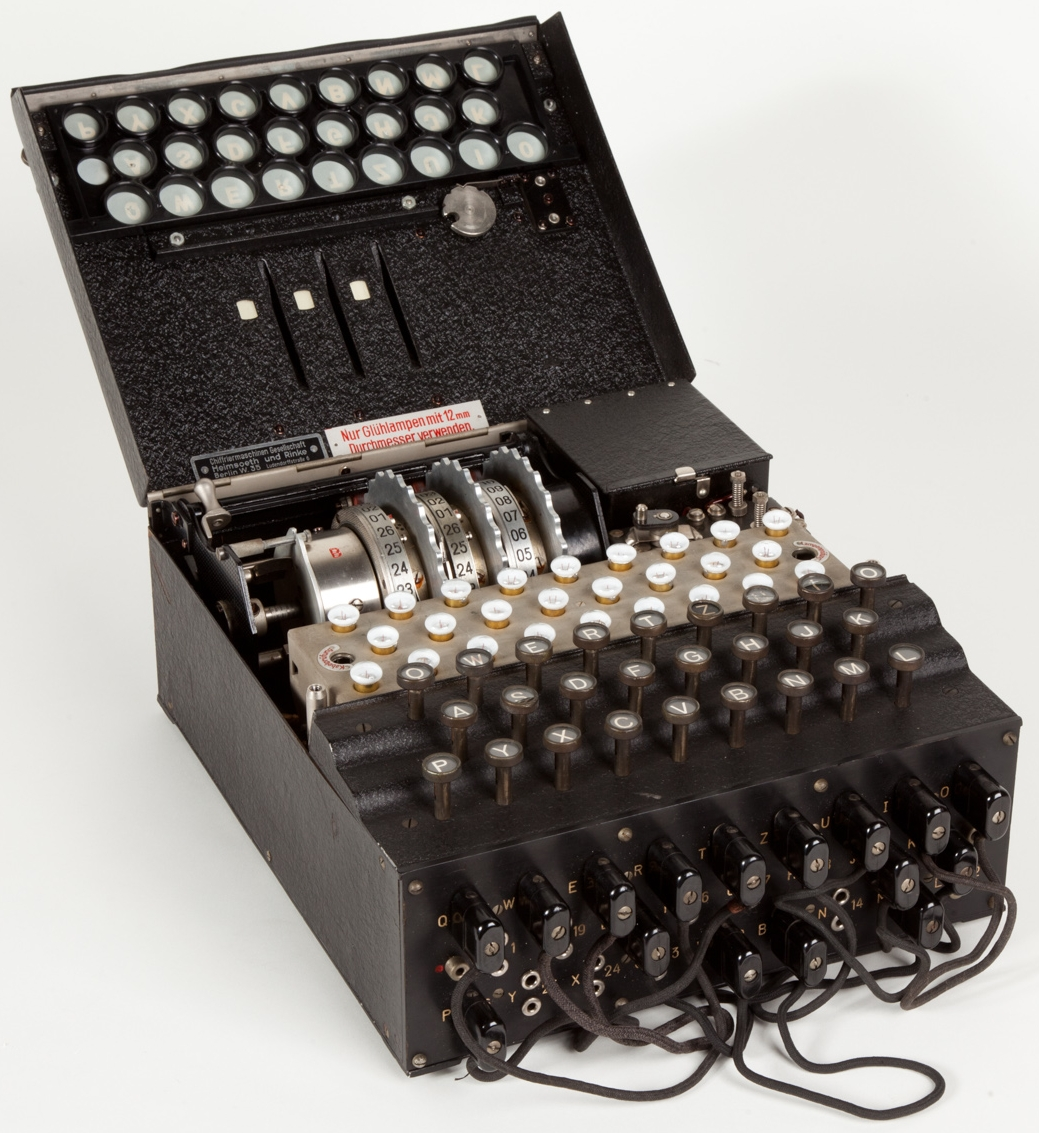
\includegraphics[scale=0.25]{wikipedia_enigmamachine.jpg}
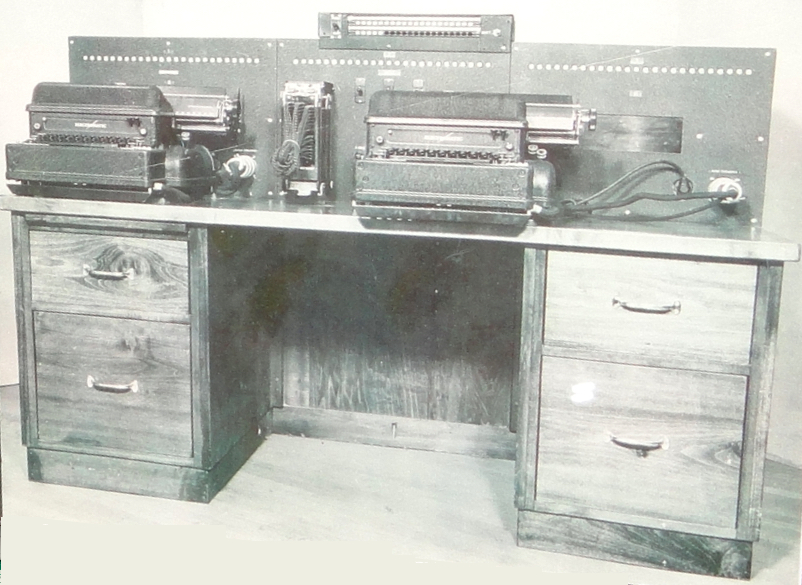
\includegraphics[scale=0.5]{wikipedia_purplemachine.jpg}
\end{frame}

\begin{frame}{Current Symmetric Cryptography: AES-256}
\begin{itemize}
    \item 256-bit key
    \item 128-bit block
    \item 14 rounds of encryption
    \item substitution, transposition, mixing
    \item \url{https://www.cryptool.org/en/cto/aes-animation}
\end{itemize}
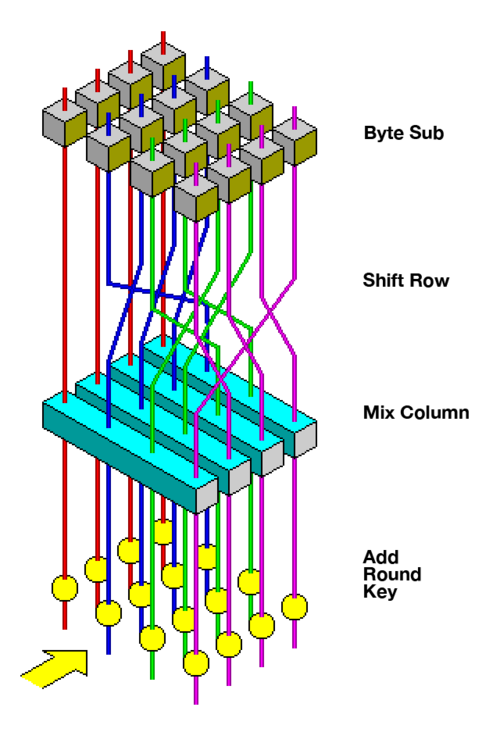
\includegraphics[scale=0.2]{aes256.png}
\end{frame}

\begin{frame}{Increasing Difficulty: CBC}
    \begin{itemize}
        \item Even with a complicated function, a key is not safe if it is reused a lot
        \item Methods of increasing difficulty: Cypher Block Chaining (CBC)
        \item Even CBC is subject to plaintext attack
    \end{itemize}
    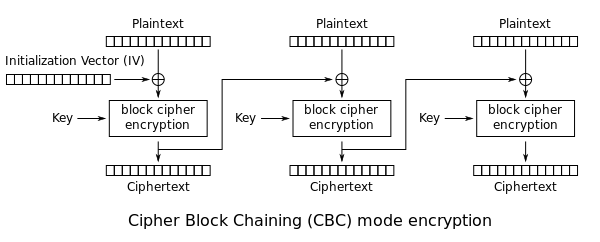
\includegraphics[scale=0.25]{CBC.png}
\end{frame}

\begin{frame}{Brute Force Attacks on AES-256}
\begin{itemize}
    \item How hard is a brute force attack?
    \item 256-bit key: $2^{256} = 1.1 x 10^{77}$
    \item Additionally the data is 128 bits
    \item Even trying $10^9$ keys per second, tiny probability of working
    \item Seems effective against computers for the next 10-20 years
\end{itemize}
\end{frame}

\begin{frame}{How much Faster Have Computers Gotten?}
\begin{itemize}
    \item Moore's law: computer circuits double every 18 to 24 months
    \item Hanging in, but speed has not been increasing at the same related
    \item Still, if the problem can be split into parallel chunks...
\end{itemize}
\includegraphics[width=10cm]{mooreslaw.pdf}
\end{frame}


\begin{frame}{Asymmetric Cryptography}
\begin{itemize}
    \item 1969: proposed asymmetric cryptography
    \item Everyone knows the public keys, can be distributed
    \item Source of public keys must be trustworthy
    \item Generally slower than symmetric cryptography operations
    \item Relies on one-way functions
    \item $m' =E(m, k_{pub})$
    \item $m = D(m', k_{priv})$
    \item E and D are inverse operators
    \item $E(D(m, k_{pub}), k_{priv}) = m$
    \item $D(E(m, k_{pub}), k_{priv}) = m$
\end{itemize}
\end{frame}

\begin{frame}{Asymmetric Cryptography}
    \begin{itemize}
        \item Public and Private key
        \item Everyone knows the public keys, can be distributed
        \item Source of public keys must be trustworthy
        \item Generally slower than symmetric cryptography operations
        \item Relies on one-way functions
        \item $m' =E(m, k_{pub})$
        \item $m = D(m', k_{priv})$
        \item E and D are inverse operators
        \item $E(D(m, k_{pub}), k_{priv}) = m$
        \item $D(E(m, k_{pub}), k_{priv}) = m$
    \end{itemize}
\end{frame}

\begin{frame}{Digital Signature}
    \begin{itemize}
        \item A digital signature proves that a message was sent by the owner of the private key
        \item Assuming
        \begin{itemize}
            \item The private key is kept secret
            \item The correct public key is distributed
            \item The cryptosystem is not broken
            \item New messages cannot be constructed with the same hash value
        \end{itemize}
        \item Compute a hash of the message: $h=H(m)$
        \item Sending the hash and the message would not work
        \item Given m, h the attacker could just change the message and rehash it
        \item Instead, send $[m, D(h, k_{priv})]$
        \item only the author knows the private key, this proves the author sent it
    \end{itemize}
\end{frame}

\begin{frame}{Signature Validate}
    \begin{itemize}
        \item Given $[m, h' = D(h, k_{priv})]$, encrypt the hash
        \item $h = E(h', k_{pub})$
        \item Compute the message hash: $h = H(m)$
        \item If the two match, the signature is valid
    \end{itemize}
\end{frame}

\begin{frame}{Proof of Identity}
    \begin{itemize}
        \item Sender picks a random number (nonce)
        \item Sender encrypts using receiver's public key $E(n, k_{pub})$ and sends
        \item Receiver decrypts: $n = D(m, k_{priv})$ and send back to sender, proving identity
        \item in ssh key authentication, both sides do this. First we verify that the server really is who it says it is
    \end{itemize}
\end{frame}

\begin{frame}{Signature Validation Security}
    \begin{itemize}
        \item Over time, the security of digital signature fades
        \item Computers get faster, and better algorithms start to threaten the hash function
        \item My idea: retain a "secret" hash on file in a secure repository
        \item If an attack in the future claims the message is not correct and offers an alternative
        \item Prove by unlocking the original secret and rehashing using the secret
    \end{itemize}
\end{frame}

\begin{frame}{Diffie-Hellman Key Exchange}
    \begin{itemize}
        \item Given RSA is vulnerable to plaintext attacks, never send known text
        \item Pick a random number (nonce)
        \item Party A computes $E(g^x \mod p, k_{pub,B})$ and sends to B
        \item Party B computes $E(g^y \mod p, k_{pub,A})$ and sends to A
        \item Both parties compute a shared key
        \item Use a symmetric algorithm (AES-256) to encrypt messages
        \item Change keys regularly (ie every 30 minutes)
    \end{itemize}
\end{frame}

\begin{frame}{Hashing}
\begin{itemize}
    \item A hash is a function that converts a sequence of bits to a number
    \item Generally, the data is far bigger than the number
    \item By definition, there are many combinations of bits that must hash to the same value
    \item Multiple values converting to the same hash value are called collisions
    \item Example: 3 bit hash value (0 .. 7)
\end{itemize}
Testing testing 123 $\rightarrow$ 1 \\
Hello there $\rightarrow$ 2         \\
Attack at dawn $\rightarrow$ 1      \\
\end{frame}

\begin{frame}{Secure Hash Algorithm}
    A cryptographic hash algorithm must:
    \begin{itemize}
        \item Any change in input should cause a large (most or all bit) change in hash
        \item Difficult to reverse engineer the message
        \item Difficult to construct a different message with the same value.
        \begin{itemize}
            \item Example
            \item hash("X sells house to Y for 1000BTC") %$\rightarrow C206AD95$
            \item hash("X gives house to Y for \$1")     %$\rightarrow C206AD95$
        \end{itemize}
    \end{itemize}
    Given m is large, there must be multiple m for the same $hash(m)$
%    \href{https://brilliant.org/wiki/secure-hashing-algorithms/}
\end{frame}

\begin{frame}{Certificates and Authorities}
    \begin{itemize}
        \item Asymmetric cryptography is convenient because it simplifies establishing secret communication, but..
        \item It does require getting the right public key
        \item Problem: Who do you trust?
        \item Solution: A Certificate Authority
        \item One place that stores all public keys and gives them out
    \end{itemize}
\end{frame}


\begin{frame}{RSA}
    \begin{itemize}
        \item RSA is an asymmetric cryptosystem using prime factorization as the one-way function
        \item Relies on the fact that
        \begin{itemize}
            \item It is easy to multiply two numbers, even big ones
            \item Very hard to factor a large number into two primes
            \item The problem is, just because we don't know how to do it does not mean it can't be done
        \end{itemize}
    \end{itemize}
\end{frame}

\begin{frame}{RSA Details}
    \begin{itemize}
        \item Pick two large primes $p=17, q=41$
        \item Compute the product $n = p q$
        \item Compute $ \phi(n) = ( p-1 )( q-1 ) = 16*40 = 640$
        \item Pick an integer $1 < e < \phi(n)$ and $e, \phi(n)$ are coprime
        \item $e = 11$
        \item Compute multiplicative inverse $d e \mod \phi(n) = 1$
        \item $d = 7$
        \item public key = $( n, e )$
        \item private key = $( n, d )$
        \item Security of RSA depends on: factoring $n$ is slow
    \end{itemize}
\end{frame}

\begin{frame}[fragile]{Extended Euclid}
\begin{lstlisting}[language=c++,mathescape=true]
extended_gcd(a, b)
  oldr $\gets$ a
  r $\gets$ b
  olds $\gets$ 1
  s $\gets$ 0
  oldt $\gets$ 0
  t $\gets$ 1
  while r $\neq$ 0 do
    quotient $\gets$ oldr $\div$ r
    oldr $\gets$ r
    r $\gets$ oldr - quotient * r
    olds $\gets$ oldt
    oldt $\gets$ t
    t $\gets$ olds - quotient * t
  end
  return olds
\end{lstlisting}    
\end{frame}

\begin{frame}[fragile]{Extended Euclid}
    Example: extendedGCD(240,46)
\begin{tabular}{p{0.8cm}|p{2cm}|p{2cm}|p{2cm}|p{2cm}} %    \hline
step & quotient       & remainder            & $s_i$            & $t_i$             \\     
0    &                & 240                  & 1                & $0$               \\ 
1    &                & 46                  & $0$               & $1$               \\   
2    & $240 / 46 = 5$ & $240 - 5 * 46 = 10$ & $1 - 5*0 = 1$     & $0 - 5*1 = -5$    \\ 
3    & $46 / 10 = 4$  & $46 - 4 * 10 = 6$   & $0 - 4*1 = -4$    & $1 - 4*(-5) = 21$ \\
4    & $10 / 6 = 1$   & $10 - 1 * 6 = 4$    & $1 - 1*-4 = 5$    & $-5 - 1*21 = -26$ \\
5    & $6 / 4 = 1$    & $6 - 1 * 4 = 2$     & $-4 -1*5 = -9$    & $21 - 1*-26 = 47$ \\
6    & $4 / 2 = 2$    & $4 - 2 * 2 = 0$     & $5 - 2*-9 = 23$ & $-26 - 2*47 = -120$ \\
\end{tabular}
$gcd = a s_i + b t_i = 240*-9 + 46*47 = 2$
\end{frame}

%\begin{frame}[fragile]{Extended Euclid}
%    Example: extendedGCD(640,11, x, y)
%\begin{tabular}{p{0.8cm}|p{2cm}|p{2cm}|p{2cm}|p{2cm}} %    \hline
%step & quotient       & remainder            & x                & y                 \\     
%0    & 640            & 11                   & 1                & 0                \\ 
%2    & $640 / 11 = 5$ & $640 \mod 11 = 10$ & $1 - 5*0 = 1$     & $0 - 5*1 = -5$    \\ 
%3    & $46 / 10 = 4$  & $46 - 4 * 10 = 6$   & $0 - 4*1 = -4$    & $1 - 4*(-5) = 21$ \\
%4    & $10 / 6 = 1$   & $10 - 1 * 6 = 4$    & $1 - 1*-4 = 5$    & $-5 - 1*21 = -26$ \\
%5    & $6 / 4 = 1$    & $6 - 1 * 4 = 2$     & $-4 -1*5 = -9$    & $21 - 1*-26 = 47$ \\
%6    & $4 / 2 = 2$    & $4 - 2 * 2 = 0$     & $5 - 2*-9 = 23$ & $-26 - 2*47 = -120$ \\
%\end{tabular}
%$gcd = a s_i + b t_i = 240*-9 + 46*47 = 2$
%\end{frame}

\begin{frame}{Asymmetric Operations in RSA}
    \begin{itemize}
        \item Encryption $c = E[m] = m^e \mod n$
        \item Decryption $m = D[c] = c^d \mod n$
        \item Secure Hash Algorithms  $hash(m) = H[m]$ \url{https://sha256algorithm.com/}
        \item Signing    $m, s= D[hash(m)]$
        \item Verifying  $hash(m) = E[s]$
    \end{itemize}
\end{frame}

\begin{frame}{Risks to RSA}
    \begin{itemize}
        \item Factoring $n=pq$ may not be slow
        \item One-way functions may not exist in general
              \url{https://en.wikipedia.org/wiki/One-way\_function}
              %\url{} Boaz Barak article
        \item Quantum computers of sufficient size could break RSA in polynomial time
        \item RSA can be broken with a plaintext attack
    \end{itemize}
\end{frame}

\begin{frame}{Elliptic Curve Cryptography: ECC}
    \begin{itemize}
        \item Elliptic Curves
        \item key generation: random 256-bit integer
        \item public key: pairs of integer coordinates on the curve (x,y)
        \item compressed public key: x coordinate + 1 bit (odd or even)
        \item Requires fewer bits than RSA
        \item Not all curves are secure! Use curves identified by NIST
        \item ECC is also not quantum secure!
    \end{itemize}
\end{frame}

\begin{frame}{ECC Algorithm Overview}
    \begin{itemize}
        \item ECC on an integer field means adding points is easy
        \item $y^2 = x^3 + 7 \mod 2^{256}$
        \item $P_2 = P_a + P_b$ 
        \item Doubling means calculating powers of $P$ are easy $2P_1 = P_1 + P_1$
        \item Any multiple can be achieved by adding the powers: $19P_a = 16P_a + 2P_a + 1P_a$
        \item The reverse is hard $P_1 / k$
    \end{itemize}
\end{frame}

\begin{frame}{ECC Visualized}
    \begin{itemize}
        \item NIST secp256k1 (used in bitcoin) over $GF(2^{256})$
        \item $y^2 = x^3 + 7 \mod 2^{256}$
        \item $p = 2^{256} - 2^{32} - 977$
        \item $G =$
          $( 0x6B17D1F2E12C4247F8BCE6E563A440F277037D812DEB33A0F4A13945D898C296,$ \\
          $  0x4FE342E2FE1A7F9B8EE7EB4A7C0F9E162BCE33576B315ECECBB6406837BF51F5 )$
    \end{itemize}
\end{frame}

\begin{frame}{ECC Discrete Logarithm Visualization}
    \begin{itemize}
        \item \url{https://cryptobook.nakov.com/asymmetric-key-ciphers/elliptic-curve-cryptography-ecc}
        \item \url{https://www.desmos.com/calculator/ialhd71we3}
    \end{itemize}
    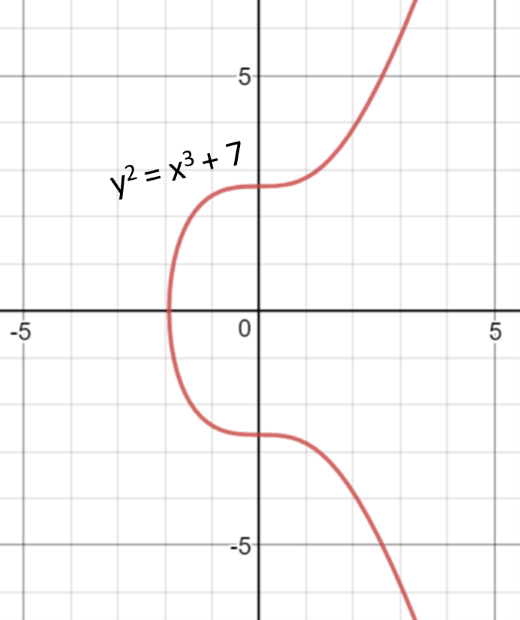
\includegraphics[scale=0.25]{ecc_secp256k1.png}
\end{frame}

\begin{frame}{ECC Discrete Logarithm Points}
    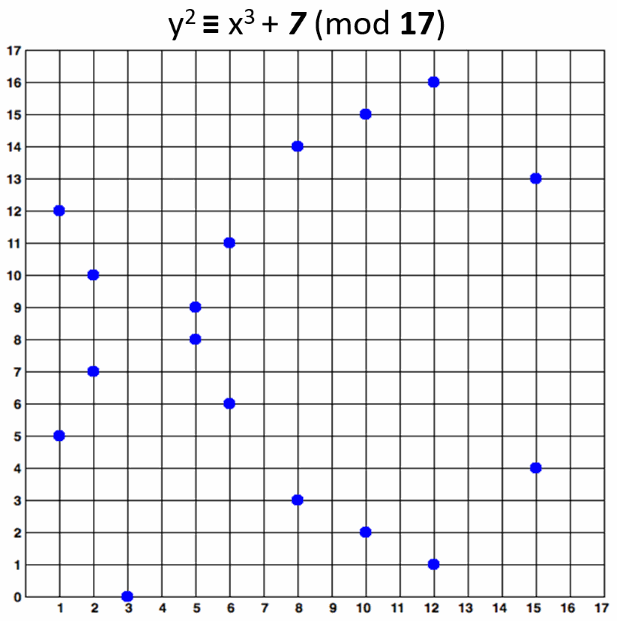
\includegraphics[scale=0.25]{ECC_mod17.png}
\end{frame}

\begin{frame}{ECC Animation}
    \url{https://curves.xargs.org/}
\end{frame}


\begin{frame}{Applications}
\begin{itemize}
    \item Blockchain: A ledger where each entry is cryptographically signed
    \begin{itemize}
        \item Finance
        \item Medicine
    \end{itemize}
    \item Smart Contracts: a program executed on a blockchain where the code defines the deal
    \item Internet of Things: devices should communicate encrypted (why?)
\end{itemize}
Can you see attacks on any of these concepts?
\end{frame}



\begin{frame}{Cryptographic Hash Functions}
    \begin{itemize}
        \item Cryptographic hash functions are algorithms that take an input (or message) and produce a fixed-size string of bytes.
        \item Properties of cryptographic hash functions include determinism, pre-image resistance, second pre-image resistance, and collision resistance.
        \item In blockchain, hash functions are used to create digital fingerprints of data, ensuring data integrity and immutability.
    \end{itemize}
\end{frame}

\begin{frame}{Secure Hash Algorithms (SHA)}
    \begin{itemize}
        \item The Secure Hash Algorithms (SHA) are a family of cryptographic hash functions designed by the National Security Agency (NSA) and published by the National Institute of Standards and Technology (NIST).
        \item SHA-256 is commonly used in blockchain to create unique hash values for blocks and transactions.
        \item SHA algorithms provide strong collision resistance and are widely adopted for securing data in blockchain networks.
    \end{itemize}
\end{frame}

\begin{frame}{Digital Signatures in Blockchain}
    \begin{itemize}
        \item Digital signatures are cryptographic mechanisms that provide authentication, integrity, and non-repudiation for digital messages or documents.
        \item In blockchain, digital signatures are used to verify the authenticity of transactions and ensure that they have been authorized by the rightful owner of the associated private key.
        \item Digital signatures rely on asymmetric cryptography, where a private key is used to sign the message and a corresponding public key is used to verify the signature.
    \end{itemize}
\end{frame}

\begin{frame}[fragile]{Elliptic Curve Cryptography (ECC)}
    \begin{itemize}
        \item Elliptic Curve Cryptography (ECC) is a form of public key cryptography based on the algebraic structure of elliptic curves over finite fields.
        \item ECC offers equivalent security to RSA and other cryptographic systems but with smaller key sizes, making it more efficient for constrained environments like blockchain.
        \item ECC is widely used in blockchain for generating key pairs, digital signatures, and key exchange protocols.
    \end{itemize}

    \includesvg{ellipticcurve.svg}

    \includesvg{ellipticcurvecryptography.svg}
\end{frame}

\begin{frame}[fragile]{Merkle Trees and Merkle Proof}
    \begin{itemize}
        \item Merkle trees are data structures that enable efficient and secure verification of large datasets.
        \item In blockchain, Merkle trees are used to summarize the transaction history within a block, allowing for quick verification of individual transactions.
        \item Merkle proofs provide a compact way to prove the inclusion or absence of a particular transaction in a block without revealing the entire block's contents.
    \end{itemize}
    \includesvg{merkletree.svg}
\end{frame}

\begin{frame}[fragile]{Public Key Infrastructure (PKI)}
    \begin{itemize}
        \item Public Key Infrastructure (PKI) is a set of hardware, software, policies, and standards used to manage digital certificates and public-private key pairs.
        \item In blockchain, PKI enables the secure issuance, distribution, and revocation of digital certificates, facilitating secure communication and transaction validation.
        \item PKI plays a crucial role in establishing trust and authenticity within blockchain networks.
    \end{itemize}
    \includesvg{pki.svg}
\end{frame}

\begin{frame}{Consensus Algorithms in Blockchain}
    \begin{itemize}
        \item Consensus algorithms are protocols used to achieve agreement among distributed nodes in a blockchain network.
        \item Common consensus algorithms include
        \begin{itemize}
            \item Proof of Work (PoW)
            \item Proof of Stake (PoS)
            \item Delegated Proof of Stake (DPoS)
            \item Practical Byzantine Fault Tolerance (PBFT)
        \end{itemize}
        \item Consensus algorithms ensure the integrity and security of the blockchain by enabling decentralized decision-making and preventing double-spending attacks.
    \end{itemize}
\end{frame}

\begin{frame}{Byzantine Fault Tolerance (BFT)}
    \begin{itemize}
        \item BFT is a property of distributed systems that can tolerate the failure of a certain number of nodes or malicious actors.
        \item In blockchain, BFT consensus algorithms ensure that the network remains operational and secure even in the presence of faulty or malicious nodes.
        \item BFT algorithms use redundancy and cryptographic mechanisms to achieve consensus and prevent Byzantine failures.
    \end{itemize}
\end{frame}

\begin{frame}{Smart Contracts and Solidity}
    \begin{itemize}
        \item Smart contracts are self-executing contracts with the terms of the agreement directly written into code.
        \item Solidity is a high-level programming language used to write smart contracts on blockchain platforms like Ethereum.
        \item Smart contracts enable decentralized applications (DApps) to automate and enforce the execution of agreements, transactions, and other processes without the need for intermediaries.
        \item Solidity, part of Ethereum is the most widely used programming language for smart contracts.
    \end{itemize}
\end{frame}

\begin{frame}{Solidity}
    \begin{itemize}
        \item Solidity is a contract-oriented, high-level programming language for implementing smart contracts
        \item Based on C++, Python and JavaScript
        \item Targets the Ethereum Virtual Machine (EVM)
        \item EVM is designed to run untrusted code by computers all over the world
        \item docs: \url{https://solidity.readthedocs.io/}
        \item Tutorial: \url{https://www.tutorialspoint.com/solidity/index.htm}
    \end{itemize}
\end{frame}

\begin{frame}{Solidity Example}

\end{frame}


\begin{frame}{Smart Contract Attacks (Solidity)}
    \begin{itemize}
        \item The code is your contract
        \item Re-entrancy Attack
              Possibility to call a function multiple times before it has completed
        \item Default Visibilities
              Functions used internally should not be visible (and callable) to the outside world
        \item Arithmetic under/overflows
        \item Entropy Illusion
        \item Race Conditions
        \item Denial of Service
    \end{itemize}
    \url{https://hacken.io/discover/most-common-smart-contract-attacks/}
\end{frame}

\begin{frame}{Famous Smart Contract Failures}
    \begin{itemize}
        \item The reentrancy attack led to hundreds of millions of dollars in losses
        \item Ethereum fork in 2016 to change the code and rewrite history
        \item DAO Hack 2016 \$60 million
        \item [Codeium hallucination!] OpenZeppelin 2019 \$100 million 
        \item Grim Finance 2021 \$30 million
        \item DFORECE Apr 2020 \$24 million
    \end{itemize}
\end{frame}

\begin{frame}{DAO Hack 2016}
    \begin{itemize}
        \item Seized 5.2 percent of ETH
        \item Required a fork of Ethereum to "fix"
        \item While the outcome may be good, effectively Ethereum is governed by an oligopoly of programmers?
        \item No court of law decides what will happen 
    \end{itemize}
\end{frame}

\begin{frame}[fragile]{Example of Reentrancy Attack}
\begin{lstlisting}
contract Bank {
  mapping (address => uint) public balances;

  function deposit() public payable{
    require(msg.value > 0, "funds needed to set balance");
    balances[msg.sender] += msg.value;
  }

  function withdraw() public {
    require(balances[msg.sender] > 0, "insufficient balance");
    (bool success, ) = msg.sender.call{value: balances[msg.sender]}("");
    require(success, "transfer failed");
    balances[msg.sender] = 0;
  }
}
\end{lstlisting}
\end{frame}

\begin{frame}[fragile]{Reentrancy Attack}
\url{https://www.infuy.com/blog/preventing-re-entrancy-attacks-in-solidity/}
contract BankAttack {
  Bank bank;

  function setBankContract(address bankContract) public {
    bank = Bank(bankContract);
  }

  fallback () external payable {
    if (address(bank).balance >= 1 ether){
      bank.withdraw();
    }
  }

  function attack() external payable {
    require(msg.value == 1 ether);
    bank.deposit{value: 1 ether}();
    bank.withdraw();
  }
}
\end{frame}

\begin{frame}[fragile]{Solution}
\begin{lstlisting}
contract Bank {
  bool private _entered;

  modifier nonReentrant {
    require(!_entered, "re-entrant call");
    _entered = true;
    _;
    _entered = false;
  }

  function withdraw() public nonReentrant { 
    require(balances[msg.sender] > 0, "insufficient balance");
    (bool success, ) = msg.sender.call{value: balances[msg.sender]}("");
    require(success, "transfer failed");
    balances[msg.sender] = 0;
  }
}
\end{lstlisting}
\end{frame}

\begin{frame}{Decentralized Applications (DApps)}
    \begin{itemize}
        \item Decentralized Applications (DApps) are software applications that run on a distributed computing system like blockchain.
        \item DApps leverage the decentralized nature of blockchain to provide transparency, security, and censorship resistance.
        \item Examples of DApps include decentralized finance (DeFi) platforms, decentralized exchanges (DEXs), and blockchain-based games.
    \end{itemize}
\end{frame}

\begin{frame}{Summary: Usefulness of Blockchain}
    \begin{itemize}
        \item Public blockchain does not appear to be useful except to criminals
        \item Being able to have multiple parties validate a blockchain so records are immutable seems to be useful
        \item Problems stem from changing technology: How do we verify the integrity of a blockchain when the cryptosystem can be broken?
        \item Cryptocurrency as an investment is speculation based on zero value
    \end{itemize}
\end{frame}

%\end{withoutheadline}
\end{document} 
